%%%%%%%%%%%%%%%%%%%%%%%%%%%%%%%%%%%%%%%%%%%%%%%%%%%%%%%%%%%%%%%
%
%     filename  = "Dissertation Index.tex",
%     version   = "Draft 1",
%     date      = "1/16/2013",
%     authors   = "Nicholas P. Nicoletti",
%     copyright = "Nicholas P. Nicoletti",
%     address   = "Department of Political Science,
%                  516 Park Hall,
%                  University at Buffalo,
%                  Buffalo, NY 14260,
%                  USA",
%     telephone = "(585) 752-5167",
%     email     = "npn@buffalo.edu",
%
%%%%%%%%%%%%%%%%%%%%%%%%%%%%%%%%%%%%%%%%%%%%%%%%%%%%%%%%%%%%%%%
%
% Change History:
%
% Draft Version 1.0 - No Changes.
%
%%%%%%%%%%%%%%%%%%%%%%%%%%%%%%%%%%%%%%%%%%%%%%%%%%%%%%%%%%%%%%%
%
% This is a template file to help get you started using the
% psuthesis.cls for theses and dissertations at Penn State
% University. You will, of course, need to put the
% psuthesis.cls file someplace that LaTeX will find it.
%
% We have set up a directory structure that we find to be clean
% and convenient. You can readjust it to suit your tastes. In
% fact, the structure used by our students is even a little
% more involved and commands are defined to point to the
% various directories.
%
% This document has been set up to be typeset using pdflatex.
% About the only thing you will need to change if typesetting
% using latex is the \DeclareGraphicsExtensions command.
%
% The psuthesis document class uses the same options as the
% book class. In addition, it requires that you have the
% ifthen, calc, setspace, and tocloft packages.
%
% The first additional option specifies the degree type. You
% can choose from:
%     Ph.D. using class option <phd>
%     M.S. using class option <ms>
%     M.Eng. using class option <meng>
%     M.A. using class option <ma>
%     B.S. using class option <bs>
%     B.A. using class option <ba>
%     Honors Baccalaureate using the option <honors>
%
% If you specify either ba or bs in addition to honors, it will
% just use the honors option and ignore the ba or bs option.
%
% The second additional option <inlinechaptertoc> determines
% the formatting of the Chapter entries in the Table of
% Contents. The default sets them as two-line entries (try it).
% If you want them as one-line entries, issue the
% inlinechaptertoc option.
%
% The class option ``honors'' should be used for theses
% submitted to the Schreyer Honors College. This option
% changes the formatting on the Title page so that the
% signatures appear on the Title page. Be sure and comment
% out the command \psusigpage when using this option since it
% is not needed and it messes up the vertical spacing on the
% Title page.
%
% The class option ``honorsdepthead'' adds the signature of the
% department head on the Title page for those baccalaureate
% theses that require this.
%
% The class option ``secondthesissupervisor'' should be used
% for baccalaureate honors degrees if you have a second
% Thesis Supervisor.
%
% The vita is only included with the phd option and it is
% placed at the end of the thesis. The permissions page is only
% included with the ms, meng, and ma options.
%%%%%%%%%%%%%%%%%%%%%%%%%%%%%%%%%%%%%%%%%%%%%%%%%%%%%%%%%%%%%%%
% Only one of the following lines should be used at a time.
\documentclass[draft,phd,12pt]{psuthesis}
%\documentclass[draft,phd,inlinechaptertoc]{psuthesis}
%\documentclass[draft,ms]{psuthesis}
%\documentclass[draft,honorsdepthead,honors]{psuthesis}
%\documentclass[draft,honors]{psuthesis}
%\documentclass[draft,secondthesissupervisor,honors]{psuthesis}
%\documentclass[draft,bs]{psuthesis}


%%%%%%%%%%%%%%%%%%%%%%%%%%%%
% Packages we like to use. %
%%%%%%%%%%%%%%%%%%%%%%%%%%%%
\usepackage{amsmath}
\usepackage{amssymb}
\usepackage{amsthm}
\usepackage{exscale}
\usepackage[mathscr]{eucal}
\usepackage{bm}
\usepackage{eqlist} % Makes for a nice list of symbols.
\usepackage[final]{graphicx}
\usepackage[dvipsnames]{color}
\DeclareGraphicsExtensions{.pdf, .jpg, .png}
\usepackage{natbib}
\usepackage{har2nat}
\usepackage{verbatim}
\usepackage{url}
\usepackage{longtable}
\usepackage{mathpazo}
\usepackage{pstricks}
\usepackage{sgamevar}
\usepackage{egameps}
\def\citeapos#1{\citeauthor{#1}'s \citeyear{#1}}
\newenvironment{my_enumerate}
{\begin{enumerate}
  \setlength{\itemsep}{1pt}
  \setlength{\parskip}{0pt}
  \setlength{\parsep}{0pt}}{\end{enumerate}}
\newenvironment{my_itemize}
{\begin{itemize}
  \setlength{\itemsep}{1pt}
  \setlength{\parskip}{0pt}
  \setlength{\parsep}{0pt}}{\end{itemize}}


%%%%%%%%%%%%%%%%%%%%%%%%
% Setting for fncychap %
%%%%%%%%%%%%%%%%%%%%%%%%
% Comment out or remove the next two lines and you will get
% the standard LaTeX chapter titles. We like these A LOT
% better.
\usepackage[Lenny]{fncychap}
\ChTitleVar{\Huge\sffamily\bfseries}


%%%%%%%%%%%%%%%%%%%%%%%%%%%%%%%
% Use of the hyperref package %
%%%%%%%%%%%%%%%%%%%%%%%%%%%%%%%
%
% This is optional and is included only for those students
% who want to use it.
%
% To use the hyperref package, uncomment the following line:
\usepackage[colorlinks]{hyperref}
%
% Note that you should also uncomment the following line:
\renewcommand{\theHchapter}{\thepart.\thechapter}
%
% to work around some problem hyperref has with the fact
% the psuthesis class has unnumbered pages after which page
% counters are reset.


%%%%%%%%%%%%%%%%%%%%%%%%%%%%%%%%%%%%
% SPECIAL SYMBOLS AND NEW COMMANDS %
%%%%%%%%%%%%%%%%%%%%%%%%%%%%%%%%%%%%
% Place user-defined commands below.



%%%%%%%%%%%%%%%%%%%%%%%%%%%%%%%%%%%%%%%%%
% Renewed Float Parameters              %
% (Makes floats fit better on the page) %
%%%%%%%%%%%%%%%%%%%%%%%%%%%%%%%%%%%%%%%%%
\renewcommand{\floatpagefraction}{0.85}
\renewcommand{\topfraction}      {0.85}
\renewcommand{\bottomfraction}   {0.85}
\renewcommand{\textfraction}     {0.15}

% ----------------------------------------------------------- %

%%%%%%%%%%%%%%%%
% FRONT-MATTER %
%%%%%%%%%%%%%%%%
% Title
\title{Politicizing War \\ \emph{Information, Democracy, and Public Opinion}}

% Author and Date of Degree Conferral or Defense
\author{Nicholas P. Nicoletti}
% the degree will be conferred on this date
\degreedate{May 2013}
% year of your copyright. I have removed this from the cover page because UB's guidelines do not include it.
\copyrightyear{2013}

% This is the document type. For example, this could also be:
%     Comprehensive Document
%     Thesis Proposal
\documenttype{Disseration}
%The department where you will be submitting the document%
\dept{Department of Political Science}
% This will generally be The Graduate School, though you can
% put anything in here to suit your needs. This has also been removes from the cover page via the psuthesis.cls document because UB guidelines do not allow for it.
\submittedto{The Graduate School}


%%%%%%%%%%%%%%%%%%
% Signatory Page %
%%%%%%%%%%%%%%%%%%
% You can have up to 7 committee members, i.e., one advisor
% and up to 6 readers.
%
% Begin by specifying the number of readers.
\numberofreaders{3}


% Input reader information below. The optional argument, which
% comes first, goes on the second line before the name.
\advisor[Thesis Advisor, Chair of Committee]
        {Phil Arena}
        {Professor of Political Science}

\readerone[Committee Member, Department Chair]
          {Harvey Palmer}
          {Professor of Political Science}

\readertwo[Committee Member]
          {Michelle A. Benson}
          {Professor of Political Science}

\readerthree[Committee Member]
            {Joshua Dyck}
            {Professor of Political Science}

\readerfour[Optional Title Here]
           {Reader Name}
           {Professor of SomeThing}

\readerfive[Optional Title Here]
           {Reader Name}
           {Professor of SomeThing}

% Makes use of LaTeX's include facility. Add as many chapters
% and appendices as you like.
\includeonly{%
Chapter-1/Chapter-1,%
Chapter-2/Chapter-2,%
Chapter-3/Chapter-3,%
Chapter-4/Chapter-4,%
Chapter-5/Chapter-5,%
Appendix-A/Appendix-A,%
Appendix-B/Appendix-B%
}

%%%%%%%%%%%%%%%%%
% THE BEGINNING %
%%%%%%%%%%%%%%%%%
\begin{document}
%%%%%%%%%%%%%%%%%%%%%%%%
% Preliminary Material %
%%%%%%%%%%%%%%%%%%%%%%%%
% This command is needed to properly set up the frontmatter.
\frontmatter

%%%%%%%%%%%%%%%%%%%%%%%%%%%%%%%%%%%%%%%%%%%%%%%%%%%%%%%%%%%%%%
% IMPORTANT
%
% The following commands allow you to include all the
% frontmatter in your thesis. If you don't need one or more of
% these items, you can comment it out. Most of these items are
% actually required by the Grad School -- see the Thesis Guide
% for details regarding what is and what is not required for
% your particular degree.
%%%%%%%%%%%%%%%%%%%%%%%%%%%%%%%%%%%%%%%%%%%%%%%%%%%%%%%%%%%%%%
% !!! DO NOT CHANGE THE SEQUENCE OF THESE ITEMS !!!
%%%%%%%%%%%%%%%%%%%%%%%%%%%%%%%%%%%%%%%%%%%%%%%%%%%%%%%%%%%%%%

% Generates the signature page. This is not bound with your
% thesis.
%\psusigpage

% Generates the title page based on info you have provided
% above.
\psutitlepage

%Generates Copyright Page
\copyrightpage{SupplementaryMaterial/Copyright}

\newpage
% Generates the committee page -- this is bound with your
% thesis. If this is an baccalaureate honors thesis, then
% comment out this line.
\psucommitteepage

% Generates the Epigraph/Dedication. The first argument should
% point to the file containing your Epigraph/Dedication and
% the second argument should be the title of this page.
\thesisdedication{SupplementaryMaterial/Dedication}{Dedication}

% Generates the Acknowledgments. The argument should point to
% the file containing your Acknowledgments.
\thesisacknowledgments{SupplementaryMaterial/Acknowledgments}

% Generates the Table of Contents
\thesistableofcontents

% Generates the List of Tables
\thesislistoftables

% Generates the List of Figures
\thesislistoffigures

% Generates the List of Symbols. The argument should point to
% the file containing your List of Symbols.
\thesislistofsymbols{SupplementaryMaterial/ListOfSymbols}

% Generates the abstract. The argument should point to the
% file containing your abstract.
\thesisabstract{SupplementaryMaterial/Abstract}


%%%%%%%%%%%%%%%%%%%%%%%%%%%%%%%%%%%%%%%%%%%%%%%%%%%%%%
% This command is needed to get the main part of the %
% document going.                                    %
%%%%%%%%%%%%%%%%%%%%%%%%%%%%%%%%%%%%%%%%%%%%%%%%%%%%%%
\thesismainmatter

%%%%%%%%%%%%%%%%%%%%%%%%%%%%%%%%%%%%%%%%%%%%%%%%%%
% This is an AMS-LaTeX command to allow breaking %
% of displayed equations across pages. Note the  %
% closing the "}" just before the bibliography.  %
%%%%%%%%%%%%%%%%%%%%%%%%%%%%%%%%%%%%%%%%%%%%%%%%%%
\allowdisplaybreaks{
%
%%%%%%%%%%%%%%%%%%%%%%
% THE ACTUAL CONTENT %
%%%%%%%%%%%%%%%%%%%%%%
% Chapters
%SourceDoc ../YourName-Dissertation.tex
\chapter{Declaration of Independence with a Really Long Title to See How it Looks When Really Long} \label{chapter1:introduction}

\section{\sloppy Modeling Techniques for Nonlinear Wave Propagation}
\citet{Gaubatz1999} developed an algorithm to investigate propagation of finite-am\-pli\-tude noise in pipes. His algorithm, based on weak shock theory, includes the effects of nonlinearity and tube wall boundary layer attenuation and dispersion. The hybrid time-frequency domain algorithm applies nonlinearity in the time domain, applies a fast Fourier transform (FFT), and then applies attenuation and dispersion in the frequency domain.  Then an inverse FFT is taken to return to the time domain to propagate to the next step.

\subsection{This is a Subsection}

We hold these truths to be self-evident, that all men are created equal,  that they are endowed by their Creator with certain unalienable Rights,  that among these are Life, Liberty and the pursuit of Happiness. --That to secure these  rights, Governments are instituted among Men, deriving their just powers  from the consent of the governed, --That whenever any Form of Government  becomes destructive of these ends, it is the Right of the People to alter  or to abolish it, and to institute new Government, laying its foundation on  such principles and organizing its powers in such form, as to them shall  seem most likely to effect their Safety and Happiness. Prudence, indeed, will dictate that Governments long established should not  be changed for light and transient causes; and accordingly all experience  hath shewn, that mankind are more disposed to suffer, while evils are  sufferable, than to right themselves by abolishing the forms to which they  are accustomed.\cite{DaviesMoon-1993-3-D-Spatial-Cha-0,Tonkin-1980-A-Basic-Attitud-0,Matsumoto-1984-A-Chaotic-Attra-0,MacKay-1988-A-Criterion-for-0,FreundNix-1996-A-Critical-Thic-0,MarsdenHolmes-1979-A-Horseshoe-in--0,Koiller-1984-A-Mechanical-Sy-0,TsiotrasLonguski-1995-A-New-Parameter-0,ShimadaNagashima-1979-A-Numerical-App-0,SmithDavenport-1988-A-Perturbation--0,Ketema-1992-A-Physical-Inte-0,GraesserCozzarelli-1994-A-Proposed-Thre-0,RichardsonMitchell-1999-A-Simplified-Va-0,MitchellRichardson-1999-A-Simplified-Va-0,Parks-1967-A-Stability-Cri-0,HsuLee-1971-A-Stability-Stu-0,BhattacharyaJames-1999-A-Theory-of-Thi-0,RimrottJanabi-Sharifi-1992-A-Torque-Free-F-0,Muller-PfeifferKranenburg-1992-A-Two-Dimension-0,HashinShtrikman-1963-A-Variational-A-0,Junkins-1997-Adventures-on-t-0}
%%%
\begin{figure}[htb]
    \centering
%    \includegraphics{\FigPath{FigureFileName}}
    \caption{CaptionText.}
    \label{ChX-figure: FigureLabel}
\end{figure}
%%%

\subsubsection{This is a Subsubsection}

We hold these truths to be self-evident, that all men are created equal,  that they are endowed by their Creator with certain unalienable Rights,  that among these are Life, Liberty and the pursuit of Happiness. --That to secure these  rights, Governments are instituted among Men, deriving their just powers  from the consent of the governed, --That whenever any Form of Government  becomes destructive of these ends, it is the Right of the People to alter  or to abolish it, and to institute new Government, laying its foundation on  such principles and organizing its powers in such form, as to them shall  seem most likely to effect their Safety and Happiness. Prudence, indeed, will dictate that Governments long established should not  be changed for light and transient causes; and accordingly all experience  hath shewn, that mankind are more disposed to suffer, while evils are  sufferable, than to right themselves by abolishing the forms to which they  are accustomed.

\section{More Declaration}

We hold these truths to be self-evident, that all men are created equal,  that they are endowed by their Creator with certain unalienable Rights,  that among these are Life, Liberty and the pursuit of Happiness. --That to secure these  rights, Governments are instituted among Men, deriving their just powers  from the consent of the governed, --That whenever any Form of Government  becomes destructive of these ends, it is the Right of the People to alter  or to abolish it, and to institute new Government, laying its foundation on  such principles and organizing its powers in such form, as to them shall  seem most likely to effect their Safety and Happiness. Prudence, indeed, will dictate that Governments long established should not  be changed for light and transient causes; and accordingly all experience  hath shewn, that mankind are more disposed to suffer, while evils are  sufferable, than to right themselves by abolishing the forms to which they  are accustomed. But when a long train of abuses and usurpations, pursuing invariably the same  Object evinces a design to reduce them under absolute Despotism, it is their  right, it is their duty, to throw off such Government, and to provide new Guards for their future security. --Such has been the patient sufferance of these Colonies; and such is now the  necessity which constrains them to alter their former Systems of Government.  The history of the present King of Great Britain [George III] is a history  of repeated injuries and usurpations, all having in direct object the  establishment of an absolute Tyranny over these States. To prove this, let Facts be submitted to a candid world. 
\chapter{Declaration of Independence 2}

\section{Introduction}
When in the Course of human events, it becomes necessary for one people  to dissolve the political bands which have connected them with another,  and to assume among the powers of the earth, the separate and equal station  to which the Laws of Nature and of Nature's God entitle them, a decent respect to the opinions of mankind requires that they should declare  the causes which impel them to the separation.

\section{More Declaration}

We hold these truths to be self-evident, that all men are created equal,  that they are endowed by their Creator with certain unalienable Rights,  that among these are Life, Liberty and the pursuit of Happiness. --That to secure these  rights, Governments are instituted among Men, deriving their just powers  from the consent of the governed, --That whenever any Form of Government  becomes destructive of these ends, it is the Right of the People to alter  or to abolish it, and to institute new Government, laying its foundation on  such principles and organizing its powers in such form, as to them shall  seem most likely to effect their Safety and Happiness. Prudence, indeed, will dictate that Governments long established should not  be changed for light and transient causes; and accordingly all experience  hath shewn, that mankind are more disposed to suffer, while evils are  sufferable, than to right themselves by abolishing the forms to which they  are accustomed. But when a long train of abuses and usurpations, pursuing invariably the same  Object evinces a design to reduce them under absolute Despotism, it is their  right, it is their duty, to throw off such Government, and to provide new Guards for their future security. --Such has been the patient sufferance of these Colonies; and such is now the  necessity which constrains them to alter their former Systems of Government.  The history of the present King of Great Britain [George III] is a history  of repeated injuries and usurpations, all having in direct object the  establishment of an absolute Tyranny over these States. To prove this, let Facts be submitted to a candid world.
\chapter{Classical SPH method}

\section{Introduction}
SPH is a mesh-free Lagragian method. In SPH, the domain is discretized by a set of particles or discretization points and the position of each particle is updated at every time step based on the motion computed. Approximation of all field variables (velocity, density and pressure, ect.) is obtained by interpolation based on discretization points. The physical laws (such as conservation laws of mass, momentum and energy) written in the form of PDEs (partial differential equations)  or ODEs (ordinary differential equations) need to be transformed into the Lagrangian particle formalism of SPH. Using a kernel function that provides the weighted estimation of the field variables at any point, the integral equations are estimated as sums over particles in a compact subdomain defined by the support of the kernel function associated with the discretization points. Thus, field variables associated to the particle are updated based on its neighbors. Each kernel function has a compact support determined by smoothing length of each particle. There are several review papers by \citet{monaghan1992smoothed, monaghan2005smoothed, rosswog2009astrophysical, price2012smoothed, monaghan2012smoothed}, giving a pretty comprehensive view over SPH. We only refer here to the representation of the constitutive equations in SPH and put more focus on specific numerical techniques for plume modeling.

\section{Fundamental principles}
There are several procedures for discretizing governing equations (PDEs or ODEs) with SPH. We present here one of them following \citet{monaghan1992smoothed, monaghan2005smoothed, monaghan2012smoothed}. The starting point of approximating a function with SPH is the translation property of the Dirac function $\delta(\textbf{x})$, for an arbitary function $A(\textbf{x})$, the following equation holds. 
\begin{equation}
A\left(\textbf{x}\right)=\int_{-\infty}^{\infty} A\left(\textbf{x} \prime\right) \delta \left(\textbf{x} \prime - \textbf{x}\right) d\textbf{x} \prime
\label{eq:Dirac-translation}
\end{equation}
The Dirac function in Eq. (\ref{eq:Dirac-translation}) can be approximated by a weighting function $w\left(\textbf{x}-\textbf{x}\prime, h\right)$ (or $w\left(\textbf{x}\prime-\textbf{x}, h\right)$) which tends to a Dirac function when the smoothing length $h \rightarrow 0$ :
\begin{equation}
\lim _{h \rightarrow 0} w\left(\textbf{x} \prime-\textbf{x}, h\right) =  \delta \left(\textbf{x} \prime - \textbf{x}\right)
\label{eq:SPH_kernel_delta}
\end{equation}
So it can be viewed as an approximate form of the Dirac function and should satisfy the normalization condition:
\begin{equation}
\int	 w\left(\textbf{x}-\textbf{x}\prime, h\right) d\textbf{x}\prime = 1
\label{eq:SPH-kernel-normalization-prop}
\end{equation}
Besides normalization, the weighting function of particle $a$ has to be symmetric with respect to $a$ to ensure that neighbor particles located at the same distance away from $a$ contribute equally to SPH summation equation, see Eq. (\ref{eq:SPH-kernel-symmetric}).
\begin{equation}
w\left(\textbf{x}- \textbf{x} \prime, h\right) = w\left(\textbf{x} \prime - \textbf{x}, h\right)
\label{eq:SPH-kernel-symmetric}
\end{equation}
The weighting function also needs to satisfy conditions such as positivity and compact support. In addition, the kernel function must be monotonically decreasing with the distance between particles.

There is a wide variety of possible weighting functions that can satisfy these requirements, such as spline functions (with different orders) and Gaussian functions. Generally, the accuracy increases with the order of the polynomials of the kernel function, but the computational cost also increases as number of interactions increase. 
We are adopting a truncated Gaussian function as the weighting function in our simulation.
\begin{equation}
w\left(\textbf{x} - \textbf{x} \prime \right) = 
\begin{cases} 
      \dfrac{1}{\left(h \sqrt{\pi}\right)^d} exp \left[- \left(\dfrac{\textbf{x} - \textbf{x} \prime}{h} \right)^2 \right] &  \vert \textbf{x} - \textbf{x} \prime \vert \leq 3h\\
      0 & \text{Otherwise}
\end{cases}
\label{eq:SPH-kernel}
\end{equation}
where $d$ is number of dimensions.
The derivative of the weighting function is:
\begin{equation}
\nabla w\left(\textbf{x} - \textbf{x} \prime \right) = 
\begin{cases} 
      -2\left(\dfrac{\textbf{x} - \textbf{x} \prime}{h}\right) \dfrac{1}{\left(h \sqrt{\pi}\right)^d} exp \left[- \left(\dfrac{\textbf{x} - \textbf{x} \prime}{h}\right)^2 \right] &  \vert \textbf{x} - \textbf{x} \prime \vert \leq 3h\\
      0 & \text{Otherwise}
\end{cases}
\label{eq:SPH-kernel-gradient}
\end{equation}

By replacing $\delta$ function in Eq. (\ref{eq:SPH_kernel_delta}) with the kernel function $w$, an arbitrary function $A\left(\textbf{x}\right)$ can then be approximated by:
\begin{equation}
A\left(\textbf{x}\right) \approx <A\left(\textbf{x}\right)> = \int_{\Omega} A\left(\textbf{x} \prime\right) w\left(\textbf{x}-\textbf{x}\prime, h\right) d\textbf{x}\prime + O\left(h^2\right)
\label{eq:SPH-fundamental-principle}
\end{equation}
As the weighting function is symmetric (Eq. (\ref{eq:SPH-kernel-symmetric})) and satisfies the normalization condition (Eq. (\ref{eq:SPH-kernel-normalization-prop})), odd error terms in Eq. (\ref{eq:SPH-fundamental-principle}) vanishe leading to a second order approximation. However, in practice, second order of accuracy can not be achieved because there is no guarantee on the symmetry of particle distribution in real simulation \citep{price2012smoothed}.
Recall that $d\textbf{x}\prime = \dfrac{dm (\textbf{x} \prime)}{\rho (\textbf{x} \prime)}$, the integration equation, Eq. (\ref{eq:SPH-fundamental-principle}), can be approximated by summation and lead to an approximation of the function $A$:
\begin{equation}
<A\left(\textbf{x}\right)> \approx \sum_b m_b \dfrac{A_b}{\rho_b} w\left(\textbf{x}-\textbf{x}_b, h\right)
\label{eq:SPH-approximation-sum}
\end{equation}
where the summation is over all the particles within the region of compact support (See Eq. (\ref{eq:SPH-kernel})) of the weighting function. 
Gradient terms may be straightforwardly calculated by taking the derivative of Eq. (\ref{eq:SPH-approximation-sum}), giving
\begin{equation}
\begin{split}
<\nabla A\left(\textbf{x}\right)> & = \dfrac{\partial }{\partial \textbf{x}} \int_{\Omega} A\left(\textbf{x} \prime\right) w\left(\textbf{x}-\textbf{x}\prime, h\right) d\textbf{x}\prime + O\left(h^2\right) \\
& \approx \sum_b m_b \dfrac{A_b}{\rho_b} \nabla w\left(\textbf{x} - \textbf{x}_b, h\right)
\end{split} 
\label{eq:SPH-scalar-function-gradient}
\end{equation}
For vector quantities the expressions are similar, simply replacing $A$ with $\textbf{A}$ in Eq. (\ref{eq:SPH-approximation-sum}) and Eq. (\ref{eq:SPH-scalar-function-gradient}), giving
\begin{align}
<\textbf{A}\left(\textbf{x}\right)> \approx \sum_b m_b \dfrac{\textbf{A}_b}{\rho_b} w\left(\textbf{x}-\textbf{x}_b, h\right) \\
<\nabla \cdot \textbf{A}\left(\textbf{x}\right)> \approx \sum_b m_b \dfrac{\textbf{A}_b}{\rho_b} \cdot \nabla w\left(\textbf{x} - \textbf{x}_b, h\right) \\
<\nabla \times \textbf{A}\left(\textbf{x}\right)> \approx \sum_b m_b \dfrac{\textbf{A}_b}{\rho_b} \times \nabla w\left(\textbf{x} - \textbf{x}_b, h\right) \\
<\nabla^j \textbf{A}^i\left(\textbf{x}\right)> \approx \sum_b m_b \dfrac{\textbf{A}_b^i}{\rho_b} \nabla^j w\left(\textbf{x} - \textbf{x}_b, h\right) 
\label{eq:SPH-vecctor-function}
\end{align}

\section{Artificial Viscosity} \label{sec:artificial-viscosity}
In classical SPH, shock waves are handled by introducing artificial viscosity, a term that is defined based on second derivatives of velocity, to smear out discontinuities. As in the case of first order derivatives, second order derivatives can be estimated by differentiating a SPH interpolation twice. However, such a formulation has two disadvantages: first, it is very sensitive to irregular distribution of particles, second, the second derivative of the kernel can change sign and lead to unphysical representations (for example, viscous dissipation causes decrease of the entropy). 

One of the most commonly used models of artificial viscosity \citep{monaghan1983shock} is:
\begin{equation}
\Pi_{ab}=- \frac{\nu}{\bar{\rho}_{ab}} \dfrac{ \textbf{v}_{ab} \cdot \textbf{x}_{ab}}{\textbf{x}_{ab}^2 + \left(\eta h\right)^2}
\label{eq:art-vis-original}
\end{equation}
The coefficient $\nu$ is defined as:
\begin{equation}
\nu = \alpha \bar{h}_{ab} \bar{c}_{ab}
\end{equation}
where 
\begin{align}
\bar{c}_{ab} = \dfrac{c_a + c_b}{2} \\
\bar{\rho}_{ab} = \dfrac{\rho_a + \rho_b}{2} \\
\textbf{v}_{ab}=\textbf{v}_a-\textbf{v}_b \\
\textbf{x}_{ab}=\textbf{x}_a-\textbf{x}_b
\end{align}
The artificial viscosity term $\Pi_{ab}$ is a Galilean invariant and vanishes for rigid rotation. It produces a repulsive force between two particles when they are approaching each other and an attractive force when they are receding from each other. 

The SPH viscosity can be related to a continuum viscosity by converting the summation to integrals \citep{monaghan2005smoothed}. It has been shown that  shear viscosity coefficient $\eta = \frac{\rho \alpha h c}{8} $ and bulk viscosity coefficient $ \zeta = \frac{5 \eta}{3}$ are appropriate for two dimensional flows and modified to $\eta = \frac{\rho \alpha h c}{10} $ , $ \zeta = \frac{5 \eta}{3}$ for three dimensional flows.
An extra term was added to $\nu$ considering aspects of the dissipative term in shock solutions based on Riemann solvers and lead to a new formulation of artificial viscosity. We adopt this new formulation in our simulation:
\begin{equation}
\Pi_{ab}^{\beta} = 
\begin{cases} 
      \dfrac{- \alpha \mu_{ab} \bar{c}_{ab} + \beta \mu_{ab}^2} {\bar{\rho}_{ab}} & \textbf{v}_{ab} \cdot \textbf{x}_{ab} < 0\\
      0 & \textbf{v}_{ab} \cdot \textbf{x}_{ab} > 0
\end{cases}
\label{eq:art-vis-shock}
\end{equation}
where
\begin{equation}
\mu_{ab} = \dfrac{h \textbf{v}_{ab} \cdot \textbf{x}_{ab}}{\textbf{x}_{ab}^2 + \left(\eta h\right)^2} 
\end{equation}
%$\alpha$ and $\beta$ are two parameters that are free to be adjusted for each case. 
$\alpha$ and $\beta$ are two parameters that can be adjusted for different cases.
$\alpha = 1$ and $\beta = 2$ are  recommended by Monaghan for best results. In our simulation, these two parameters are calibrated to  $\alpha = 0.3$ and $\beta = 0.6$. $\eta$ is usually taken as 0.1 to prevent singularities.
%when $\textbf{x}_{ab} = 0$.

\section{Discretization of governing equations and extensibility}
The basic interpolation given in Eq. (\ref{eq:SPH-approximation-sum}) to Eq. (\ref{eq:SPH-vecctor-function}) provides a general way to obtain SPH expressions of governing equations. The problem is that using these expressions ``{as is}" in general leads to quite poor gradient estimates. Various tricks can be used to conserve linear and angular momentum and thermal energy \citep{monaghan1992smoothed}. Special treatments are also needed for second order derivative terms \citep{monaghan2005smoothed}. We only refer here to one of these possible discretizations of compressible Euler equations with SPH:
\begin{align}
<\rho_a> = \sum_b m_b w_{ab} \left(h\right) \label{eq:ns-sph-d} \\
\left\langle\dfrac{d \textbf{v}_a}{d t}\right\rangle = -\sum_b m_b \left(\dfrac{p_b}{\rho_b^2} + \dfrac{p_a}{\rho_a^2} + \Pi_{ab}\right) \nabla_a w_{a b}\left(h\right) +\textbf{g} \label{eq:ns-sph-v} \\
\left\langle\dfrac{d e_a}{d t}\right\rangle=
 0.5\sum_b m_b \textbf{v}_{a b}\left(\dfrac{p_b}{\rho_b^2} + \dfrac{p_a}{\rho_a^2} + \Pi_{ab}\right) \cdot \nabla_a w_{a b}\left(h\right) \label{eq:ns-sph-e}
\end{align}
where, $a$ is the SPH particle index, $\textbf{v}_{a b} = \textbf{v}_a - \textbf{v}_b$. $\Pi$ is an artificial viscosity term, which is discussed in section \ref{sec:artificial-viscosity}. $w_{a b}\left(h\right)$ is a concise form of $w\left(\textbf{x}_a - \textbf{x}_b, h\right)$ and from here on, we will use this concise form.
%However, these discretized formulations will not guarantee conservation of entropy. We can obtain conservation of entropy by giving up on conservation of mass or thermal energy adopting  alternative discretized formulations \citep{monaghan1992smoothed}.
As a Lagrangian method, particle position is also updated at every time step.
\begin{equation}
\left\langle\dfrac{d \textbf{x}_a}{dt}\right\rangle = \textbf{v}_a \label{eq:SPH-update-pos}
\end{equation}

We highlight an important feature of the SPH methodology. Adding new physics and new phases into the model is trivial in terms of discretization. For example, adding of new source (or sink) into Eq. (\ref{eq:ns-sph-d}), adding a drag force into Eq. (\ref{eq:ns-sph-v})  and adding a heat exchange term into Eq. (\ref{eq:ns-sph-e}) leads to the new discretization form:
\begin{align}
<\rho_a> = \sum m_b w_{ab} \left(h\right) + \dot{\rho}\left(\textbf{x},t\right)\label{eq:ns-source-sph-d} \\
\left\langle\dfrac{d \textbf{v}_a}{d t}\right\rangle= -\sum_b m_b \left(\dfrac{p_b}{\rho_b^2} + \dfrac{p_a}{\rho_a^2} + \Pi_{ab}\right) \nabla_a w_{a b}\left(h\right) +\textbf{g} + D \sum	_b m_b \dfrac{\textbf{v}_b - \textbf{v}_a}{\rho_b} \label{eq:ns-drag-sph-v}
\end{align}
\begin{equation}
\begin{split}
\left\langle\dfrac{d e_a}{d t}\right\rangle
&= 0.5\sum_b m_b \textbf{v}_{a b}\left(\dfrac{p_b}{\rho_b^2} + \dfrac{p_a}{\rho_a^2} + \Pi_{ab}\right) \cdot \nabla_a w_{a b}\left(h\right) \\
&+ \sum_b \dfrac{m_b}{\rho_b}\left(\kappa_a + \kappa_b\right) \dfrac{\left(T_a - T_b\right)}{\textbf{r}_a - \textbf{r}_b} w_{ab}\left(h\right) \label{eq:ns-conduction-sph-e}
\end{split}
\end{equation}

where the source term $\dot{\rho}$ can be a "sink" of erupted vapor due to its phase change.
%(see microphysics modelling in ATHAM \citep{oberhuber1998volcanic}).
$D$ is a drag force coefficient. $\kappa$ is the heat conduction coefficient. $T$ is the temperature. Other physics can be added easily in a similar way. Adding of these new terms leads to modification of only a few lines in the source code. The drag force term should show up when dynamic disequilibrium between different phases is considered. In that case, each phase needs one set of governing equations of Navier-Stokes type. Adding of new phase into SPH code only needs adding few new lines for the new phase besides interaction terms introduced by the new phase.

\section{Time step}
The physical quantities (velocity, density and pressure) and particle position change every time step. The Courant condition, which is in spirit similar to the Courant condition for the mesh-based methods, is used to determine the time step $\Delta t$.
\begin{equation}
\Delta t = \textrm{CFL} \min_a \bigg \lbrace \dfrac{\left[\frac{m_a}{\rho_a}\right]^{\frac{1}{d}}}{c_a} \bigg \rbrace
\end{equation}
where $c_a$ is sound speed at particle $a$ and calculated based on heat specific ration of the mixture $\gamma_m$ (See Eq. (\ref{eq:sound-speed-mixture})). 
$d$ is number of dimensions. 
\begin{equation}
c_a = \left( \gamma_m \frac{p}{\rho} \right)^{0.5}
\label{eq:sound-speed-mixture}
\end{equation}

First order Euler integration, with $\textrm{CFL} = 0.2$, is used to advance in time.

\section{Tensile instability and corrected derivatives}
The classical SPH method was known to suffer from tensile instability and boundary deficiency. Tests of the standard SPH method indicate an instability in the tensile regime, while the calculations are stable in compression.  A simple example of such a test calculation exhibiting the instability involves a body which is subjected to an uniform initial stress, either compressive or tensile. If the initial stress is tensile, a very small velocity perturbation on a single particle can lead to particles clumping together, forming large voids and seriously corrupting density distribution. But if the initial stress is compressive, the small velocity perturbation on a single particle can not lead to any changes in particle distribution \citep{swegle1995smoothed}. To address these difficulties, \citep{chen1999improvement} proposed a corrected SPH formulation. For 1D case, employing a Taylor expansion for $A\left(x\right)$ about $x_a$, multiplying both sides by kernel function and then doing integration over the domain gives
\begin{equation}
\begin{split}
\int_{\Omega} A\left(x\right) w\left(x- x_a, h\right) dx 
& = A_a \int_{\Omega} w\left(x - x_a, h\right) dx \\
&+\dfrac{\partial A}{\partial x}(x_a) \int_{\Omega} \left(x-x_a\right) w\left(x - x_a, h\right) dx +...
\end{split}
\end{equation}
Ignoring derivative terms higher than first order, and writing the integral in particle approximation form leads to:
\begin{equation}
A_a = \frac{\sum_b m_b \dfrac{A_b}{\rho_b} w\left(x_a-x_b, h\right)}{\sum_b m_b \dfrac{1}{\rho_b} w\left(x_a-x_b, h\right)}
\label{eq:CSP-function-approximation-1d}
\end{equation}
Notice that the denominator in Eq. (\ref{eq:CSP-function-approximation-1d}) is actually summation approximation of Eq. (\ref{eq:SPH-kernel-normalization-prop}). That is to say, Eq. (\ref{eq:CSP-function-approximation-1d}) and Eq. (\ref{eq:SPH-approximation-sum}) are the same for particles far away from boundaries as the denominator in Eq. (\ref{eq:CSP-function-approximation-1d}) becomes $1$ in that case.
The first order derivative term can be obtained in a similar way:
\begin{equation}
\nabla A_a = \frac{\sum_b m_b \dfrac{A_b - A_a}{\rho_b} \nabla_a w\left(x_a-x_b, h\right)}{\sum_b m_b \dfrac{x_b - x_a}{\rho_b} \nabla_a w\left(x_a-x_b, h\right)}
\end{equation}

For problems of higher dimension, the expressions for function approximation are exactly the same as Eq. (\ref{eq:CSP-function-approximation-1d}), even though the derivation is different. The first order derivative can be obtained by solving system of equations explicitly or numerically \citep{chen1999improvement}.

\section{Mass fraction update}
Air and erupted material are represented by two different sets of SPH particles (or discretization points) in the model. Based on assumptions we made in section \ref{sec:physics-model}, only density needs to be updated respectively for each phase. The updating of density is exactly the same as Eq. (\ref{eq:ns-sph-d}) in spirit.  Particles of phase 1 are not be counted while evaluating density of phase 2 and vice versa. Updating of density is then based on the following discretized equations.
\begin{equation}
<\rho_{\alpha}^a>=\frac{\sum m_b w_{\alpha b} \left(h\right)}{\sum \frac{m_b}{\rho_b} w_{\alpha b} \left(h\right) +\sum \frac{m_j}{\rho_j} w_{\alpha j} \left(h\right)} \label{eq:gov-sph-d1}
\end{equation}
\begin{equation}
<\rho_\alpha^{sg}>=\frac{\sum_j m_j w_{\alpha j} \left(h\right)}{\sum \frac{m_b}{\rho_b} w_{\alpha b} \left(h\right) +\sum \frac{m_j}{\rho_j} w_{\alpha j} \left(h\right)} \label{eq:gov-sph-d2}
\end{equation}
where the subscript $a$ and $b$ represents air particles (phase 1) while $i$ and $j$ represents erupted material. $\beta$ and $\alpha$ represents either erupted material or air.
$\rho_a^a$ is density of phase 1 (air). 
 $\rho_i^{sg}$ is density of phase 2 (erupted material).
$\rho=\rho^a + \rho^{sg}$ is density of mixture of air and erupted material. 
By definition, the mass fraction is updated according to Eq. (\ref{eq:gov-sph-xi}).
\begin{equation}
<\xi_{\alpha}> = \dfrac{\rho^{sg}_{\alpha}}{\rho_{\alpha}}
\label{eq:gov-sph-xi}
\end{equation}

In areas far away from the interface, updating of density is exactly the same as that for single phase flow. For example, in the right side and left side (or blue areas) in Fig. \ref{fig:SPH-multiple-density}, where there are only air particles, Eq.  (\ref{eq:gov-sph-d2}) evaluates to zero and total density is:
\begin{equation}
\rho_{\alpha}=\rho_{\alpha}^a=\frac{\sum m_b w_{\alpha b} \left(h\right)}{\sum \frac{m_b}{\rho_b} w_{\alpha b}}
\end{equation}
Which is a special case of Eq. (\ref{eq:CSP-function-approximation-1d}). For these areas occupied by only particles of phase 2 and far away from the interface, similarly, the equation for density update becomes: 
\begin{equation}
\rho_{\alpha}=\rho_{\alpha}^{sg}=\frac{\sum m_j w_{\alpha j} \left(h\right)}{\sum \frac{m_j}{\rho_j} w_{\alpha j}}
\end{equation}
That is to say, the same density updating equation can be applied for both phases and no additional numerical treatment needed to locate where the interface is.

\begin{figure}
\center
\includegraphics[width=12cm]{Chapter-3/Figures/Interface}
\caption{In the left figure, the blue particles (phaseID=1) represent air particles the red ones (phaseID=2) represent erupted material. The right figure shows corresponding mass fraction. Mass fraction are evaluated based on Eq. (\ref{eq:gov-sph-d1}) and Eq. (\ref{eq:gov-sph-d1}) without any other interface track or capture method.}
\label{fig:SPH-multiple-density}
\end{figure}

Interface construction will become necessary and important when attempt to include the effects of mixing by resolving the detailed interface structure and dynamics of turbulence. 
As a Lagrangian method, interface tracking in SPH is explicit through capturing of the locations of the particles, much simplier than Euleruan Methods.
The existence of complex evolving interfaces between phases presents severe challenges to conventional Eulerian grid-based numerical methods. Either interface tracking (Lagrangian) \citep{harlow1965numerical, wrobel1991computational, cheng1995simplified} or interface capturing (Eulerian) \citep{hirt1981volume, youngs1982time, gerlach2006comparison, gopala2008volume} methods are used to reconstruct the flow interface of free boundary flow. High computational cost, a tendency to form numerical instabilities and the inability to track complex topological changes are the significant drawbacks of tracking techniques \citep{hirt1981volume, unverdi1992front, anderson1998diffuse}. For interface capturing (Eulerian) method, the surrendering of surface detail before the phase transport calculation means that interface reconstruction is required between time steps to recover the interface information, which needs additional numerical effort \citep{hirt1981volume, youngs1982time}.
Since SPH is able to adaptively adjust the discretization and automatically construct the interface. SPH requires less additional numerical effort for interface construction and therefore is more suitable for volcanic plume simulation.
 
%SPH is able to handle multiphase problems with less additional numerical effort for dealing with interfaces by simply tagging particles of each phase.

\section{Turbulence modeling with SPH}
For high speed shearing flow, the momentum exchange and heat transfer are dominated by turbulent fluctuations as turbulent exchange coefficients are several magnitudes larger than corresponding physical coefficients (molecular viscosity and heat conduction coefficient). In addition to momentum and enrgy exchange, mixing between plume and air is important in plume modeling. Quantifying these mixing processes in real implementation is challenging because of the scale disparity between the large-scale fluid motion and the diffusion processes on interface that ultimately lead to mixing. 
%The energy transfer between these scales occurs through turbulent motion, created either by fluid instabilities or by breaking internal waves. For volcanic plume, a shearing flow, the fluid instabilities dominated the mixing process. 
One way to include enough turbulence in the model is to use the SPH-SPS (SPH sub-particle-scale) turbulence model. 
Another way is to use fine enough resolution (namely, the direct numerical simulation method) at the expense of much higher computational cost which results from both increase in number of particles and decrease in time steps constrained by the CFL (Courant-Friedrichs-Lewy) condition. Here we choose the SPH-SPS method. Among existing SPH-SPS turbulence models \citep{holm1999fluctuation, monaghan2002sph, violeau2007numerical, monaghan2011turbulence}, we adopt a LANS type turbulence model, the $SPH-\varepsilon$ turbulence model \citep{monaghan2011turbulence}. However, the $SPH-\varepsilon$ turbulence model was proposed only for incompressible flow. In the following section, we will extend it for compressible flow. It is necessary to mention that all other existing SPH-SPS turbulence models \citep{holm1999fluctuation, monaghan2002sph, violeau2007numerical} also only focus on incompressible flow.

%Even though free surface flow are in nature turbulent, detailed research on turbulence modeling in SPH method is rather scarce. Among the first papers on turbulence are the implementations of the $\alpha$ turbulence model \citep{holm1999fluctuation, monaghan2002sph} and the RANS (Reynolds averaged Navier-Stokes) approach \citep{violeau2007numerical}. The first wall-bounded LES (large eddy simulation) simulation with SPH was performed by \citet{issa2005numerical}. An improved version of $SPH-\alpha$ method  \citep{monaghan2002sph} is proposed by \citet{monaghan2011turbulence}, which we refer to as $SPH-\varepsilon$ method. We adopt $SPH-\varepsilon$ method in our model. Most of these papers constrain their focus to incompressible flow. 
%$SPH-\alpha$ model \citep{monaghan2002sph} is a powerful extension of the XSPH algorithm which reduces disorder at short length scales and retains the constants of the motion. However, in that paper, energy conservation equation is discretized in a way that is exactly the same as usual SPH. There is no special treatment on energy conservation equation. The recent improved version \citep{monaghan2011turbulence} of $SPH-\alpha$ method focuses on incompressible flow only.
% 

\subsection{Langrangian average in $SPH-\varepsilon$}
\citet{monaghan2011turbulence} constructed $SPH-\varepsilon$ turbulence model within the framework of SPH in such a way that general principles such as conservation of energy, momentum and circulation are satisfied using the ideas associated with the LANS turbulence modeling. The basic idea of $SPH-\varepsilon$ is to determine a smoothed (averaged in space) velocity $\widehat{\textbf{v}}$ by a linear operation on the unsmoothed velocity $\textbf{v}$. The SPH particles move with this smoothed velocity and hence the average motion of the fluid is determined by the averaged velocity $\widehat{\textbf{v}}$:
\begin{equation}
\dfrac{d \textbf{x}_a}{dt} = \widehat{\textbf{v}}_a \label{eq:gov-update-pos-turbulence}
\end{equation}

Average of physical quantities over space introduces extra terms into the governing equations. Once the form of the smoothing (average) is chosen these extra terms are determined.
The typical LANS model uses a smoothed velocity $\widehat{\textbf{v}}$ 
defined in terms of the unsmoothed velocity $\textbf{v}$ by:
\begin{equation}
\widehat{\textbf{v}}\left(\textbf{x}\right)=\int \textbf{v}\left(\textbf{x} \prime\right)G\left(\vert \textbf{x} \prime - \textbf{x} \vert, l\right) d\textbf{x} \prime
\end{equation}
where $G$ satisfies:
\begin{equation}
\int G\left(\vert \textbf{x} \prime - \textbf{x} \vert, l\right) d\textbf{x} \prime =1
\end{equation}
and is a member of a sequence of functions which tends to the $\delta$ function in the limit when $ l\rightarrow 0$. A typical example is Gaussian.
The length scale $l$ determines the characteristic width of the kernel and the distance over which the velocity is smoothed.

It is a common practice in LANS to use a differential equation for the smoothing rather than the integral form and finally reach to a system of equations that need to be solved implicitly. In $SPH-\varepsilon$ method, a XSPH \citep{monaghan1989problem} smoothing is adopted which conserves linear and angular momentum. In this way, solving of a system of equations is avoided and it also makes the method simple to implement and cheap for computation. 
The discretized form of the momentum equation is obtained through lengthy derivation. Derivation and other discussions are available in the literature -- see for e.g. \citep{monaghan2011turbulence}. Here we provide a brief summary of key steps.

The smoothing adopted by \citet{monaghan2011turbulence}  is:
\begin{equation}
\widehat{\textbf{v}}\left(\textbf{x}\right)=\textbf{v}\left(\textbf{x}\right)+ \epsilon \int \left(\textbf{v}\left(\textbf{x} \prime\right)-\textbf{v}\left(\textbf{x}\right)\right)G\left(\vert \textbf{x} \prime - \textbf{x} \vert, l\right) d\textbf{x} \prime
\end{equation}
As function $G$ has the same feature as kernel function $w$, SPH approximation of the integration leads to:
\begin{equation} \label{eq:SPH-epsilon-filtering}
\widehat{\textbf{v}}\left(\textbf{x}\right)=\textbf{v}\left(\textbf{x}\right)+\epsilon \sum_b m_b \dfrac{\left(\textbf{v}_b -\textbf{v}\right)}{\rho _b} G\left(\vert \textbf{x} _b - \textbf{x} \vert, l\right)
\end{equation}
By making the replacement:
\begin{equation}
\label{eq:replacement-in-turb-derive}
\dfrac{G\left(\vert \textbf{x} _b - \textbf{x} _a \vert, l\right)}{\rho _b} \rightarrow \dfrac{K_{ab}}{M}
\end{equation}
where $K_{ab} = l^d G_{ab}$, $M = \rho_0 l^d$ in which $d$ is the dimension and $\rho_0$ is initial density. $SPH-\varepsilon$ turbulence model is obtained after lengthy derivation:
\begin{equation}
\label{eq:monaghan-mom-turb}
\dfrac{d \textbf{v}_a}{dt} = -\sum_b \left[ m_b \left(\dfrac{p_b}{\rho_b^2} + \dfrac{p_a}{\rho_a^2}\right) \bigtriangledown_aw_{a b}\left(h\right)\right] + \sum_b m_b \dfrac{\varepsilon}{2} \dfrac{\textbf{v}_{ab} \cdot \textbf{v}_{ab}}{M} \bigtriangledown_a K_{ab}
\end{equation}
Notice that if $l$ is constant: 
%Please notice that the above equation is slightly different from the original equation in Monaghan's paper (Eq. (2.17)). The original equation is based on the assumption that density is uniform initially. This assumption is not general and atmosphere density is stratified in our plume simulation. And the slight modification will not influence following derivation if $l$ is uniform and keep constant because:
%
%{\bf WE NEED TO SAY SOMETHING ABOUT INCOMPRESSIBILITY HERE}
%
\begin{equation}
\nabla K_{ab} = \nabla \left(l^d G_{ab}\right) = l^d \nabla G_{ab}
\end{equation}
The discretized momentum equation with $SPH-\varepsilon$ turbulence model can be written in terms of $G_{ab}$ instead of $K_{ab}$:
\begin{equation}
\label{eq:SPH-mom-epsilon-turb}
\dfrac{d \textbf{v}_a}{dt} = -\sum_b \left[m_b \left(\dfrac{p_b}{\rho_b^2} + \dfrac{p_a}{\rho_a^2}\right) \bigtriangledown_aw_{a b}\left(h\right)\right] + \sum_b m_b \Phi_{ab}\bigtriangledown_aG_{ab}\left(l\right)
\end{equation}
where 
\begin{equation}
\Phi_{ab}=\dfrac{\varepsilon}{2} \dfrac{\textbf{v}_{ab} \cdot \textbf{v}_{ab}}{\rho_b} 
\end{equation}
Which is the extra stress term induced by average. We take coefficient $\varepsilon$ as 0.8 following \citet{monaghan2011turbulence}.

For compressible flow, the energy equation is coupled with the momentum equation and mass conservation equation. Averaging of thermal energy over space introduces some additional terms besides the stress term induced by velocity average. \citep{NASACompressibleTurbulence}. The averaged momentum equation for compressible flow are in the same form as that for incompressible flow, all of other additional terms, besides the corresponding velocity average induced stress term, show up in the energy equation. Most turbulence modeling focuses on the stress terms induced by average of velocity. These stress terms are usually either solved directly (for example, LANS methods) or defined via a constitutive relation (for example, large eddy simulation method). Less attention is typically given to the other terms. Most commonly, a Reynolds analogy is used to model the turbulent exchange. Simulations of heat transfer, or other scalar transfer, in turbulent flow simply involve adding transport terms for thermal energy or species concentration, at the expense of greater storage and longer computing times but without other difficulties \citep{cebeci2013analysis}. We adopt this strategy. %PDAC \citep{neri2003multiparticle} also adopted a Reynolds analogy in its turbulence modeling.
The additional terms associated with molecular diffusion and turbulent transport in the energy equation are either modeled in different ways or neglected sometimes \citep{NASACompressibleTurbulence}. We neglect these terms in our simulation.

\subsection{Turbulent heat transfer}
We adopt Reynolds analogy to get the heat transfer coefficient due to turbulence.
The Prandtl number is defined as:
\begin{equation}
Pr=\dfrac{C_p \mu}{\kappa}
\end{equation}
where, $\mu$ is the dynamic viscosity, $\kappa$ is the thermal conductivity. And $\mu$  can be written in term of the absolute viscosity (kinematic viscosity) as:
\begin{align}
\mu=\rho \nu
\end{align}
Then
\begin{equation}
\kappa=\dfrac{C_p \mu}{Pr}
\end{equation}
Typical value of $Pr_t$ for air is 0.7 $\sim$ 0.9 . We take $Pr_t=0.85$ for gases as recommended \citet{kays1994turbulent} from summarizing of experimental results. 

\citet{monaghan2005smoothed} summarized the simulation of viscosity and heat conduction in his review on SPH. We will refer to his summary in our following discussion. The additional term in discretized momentum equation, Eq. (\ref{eq:SPH-mom-epsilon-turb}), is the turbulent shear stress term. 
Recall that molecular viscosity can be discretized with SPH as shown in Eq. (\ref{eq:art-vis-original}). 
It has been shown that the discretized molecular viscosity has both bulk viscosity and shear viscosity, where shear viscosity coefficient is \citep{monaghan2005smoothed}:
\begin{equation}
\nu_t = S \nu
\end{equation}
with
\begin{equation}
S= 
\begin{cases} 
      \dfrac{1}{10} & if  \quad d=3 \\
      \\
     \dfrac{1}{8}  & if  \quad d=2 
\end{cases}
\end{equation}
The turbulent viscosity coefficient can be inferred from that formulation if we can reformulate the turbulent shear stress term in a form which is similar to the molecular shear term.
Reformulating the turbulent shear stress term:
\begin{equation}
\label{eq:turb-stress-reformulate-to-artificial-vis}
 \sum_b \dfrac{\varepsilon}{2} \dfrac{m_b}{\rho_b} \textbf{v}_{ab} \cdot \textbf{v}_{ab} \nabla_a G_{ab}\left(l_a\right)= \sum_b \dfrac{\varepsilon}{2S} m_b \dfrac{\textbf{v}_{ab}}{\rho_b} \dfrac{S \textbf{v}_{ab} \cdot \textbf{x}_{ab}}{x_{ab}^2} \dfrac{x_{ab}^2}{\textbf{x}_{ab}} \nabla_a G_{ab}\left(l_a\right) 
\end{equation}
then the turbulent viscosity coefficient can be inferred from Eq. (\ref{eq:turb-stress-reformulate-to-artificial-vis}).
\begin{equation}
\nu_t = \dfrac{\varepsilon}{2S} \dfrac{\textbf{v}_{ab} \cdot \textbf{x}_{ab}}{\rho_b}
\end{equation}
Please note that turbulent viscosity term has opposite sign with molecular viscosity term in discretized momentum equation and there is a minus sign in the expression of $\Pi_{ab}$, and they cancel out.

However, the above equation is correct only for the 1D situations. For 2D or 3D, it is not easy to get an explicit expression. 
We adopt an alternative way: obtaining a value for each pair of particles instead of persisting on getting an analytical expression. Choosing the smoothing function as the same as SPH kernel and the smoothing length scale $l$ as the same as smoothing length $h$, the ratio between turbulent shear stress and physical shear stress is: 
\begin{equation}
\begin{split}
\Upsilon_{ab} &= \dfrac{\dfrac{\varepsilon}{2} \dfrac{\textbf{v}_{ab} \cdot \textbf{v}_{ab}}{\rho_b}}{\dfrac{S \nu}{\rho_{ab}} \frac{\textbf{v}_{ab} \cdot \textbf{x}_{ab}}{x_{ab}^2 + \eta^2 h_{ab}^2}} \\
 & = \dfrac{\varepsilon \left(x_{ab}^2 + \eta^2 h_{ab}^2\right)}{2 S \nu} \dfrac{\textbf{v}_{ab} \cdot \textbf{v}_{ab}}{\textbf{v}_{ab} \cdot \textbf{x}_{ab}}
\end{split}
\end{equation}
$\Upsilon_{ab}$ is essentially equivalent to the ratio between turbulent viscous effect of particle b on particle a and molecular viscous effect of particle b on particle a. Turbulent viscosity can be easily obtained by:
\begin{equation}
\begin{split}
\nu_{t,ab} &= \nu \Upsilon_{ab} \\
&= \dfrac{\varepsilon \left(x_{ab}^2 + \eta^2 h_{ab}^2\right)}{2 S} \dfrac{\textbf{v}_{ab} \cdot \textbf{v}_{ab}}{\textbf{v}_{ab} \cdot \textbf{x}_{ab}}
\end{split}
\end{equation}
The corresponding turbulent thermal conductivity should be
\begin{equation}
\kappa_{t,ab}=\dfrac{\varepsilon \overline{C_{p,ab}} \overline{\rho_{ab}} \left(x_{ab}^2 + \eta^2 h_{ab}^2\right) \textbf{v}_{ab} \cdot \textbf{v}_{ab}}{2 S Pr_t\textbf{v}_{ab} \cdot \textbf{x}_{ab}}
\end{equation}
$\overline{C_{p,ab}}$ and $\overline{\rho_{ab}}$ are simply the arithmetic means of specific heat and density. The term used to prevent singularity now can be removed. 
\begin{equation}
\kappa_{t,ab}=\dfrac{\varepsilon \overline{C_{p,ab}} \overline{\rho_{ab}} x_{ab}^2 \textbf{v}_{ab} \cdot \textbf{v}_{ab}}{2 S Pr_t\textbf{v}_{ab} \cdot \textbf{x}_{ab} }
\end{equation}
We also need to prevent singularity, so: 
\begin{equation}
\kappa_{t,ab}= 
\begin{cases} 
      0 & if  \quad \textbf{v}_{ab}=0 \quad or \quad \textbf{x}_{ab}=0 \\
      \dfrac{\varepsilon \overline{C_{p,ab}} \overline{\rho_{ab}} x_{ab}^2 \textbf{v}_{ab} \cdot \textbf{v}_{ab}}{2 S Pr_t\textbf{v}_{ab} \cdot \textbf{x}_{ab} } & \text{otherwise}
\end{cases}
\label{eq:SPH-LANS-heat-conductivity}
\end{equation}

Heat conduction equation without source term is:
\begin{equation}
C_p \dfrac{dT}{dt} = \dfrac{1}{\rho} \nabla \left(\kappa \nabla T\right)
\end{equation}
Second spatial derivative can be approximated with SPH by following \citet{monaghan2005smoothed}: 
\begin{equation}
C_p \dfrac{dT}{dt} = \sum_b \dfrac{m_b}{\rho_a \rho_b} \left(\kappa_a + \kappa_b\right) \left(T_a - T_b\right) F_{ab} \left(h\right)
\end{equation}
where $F_{ab} (h)$ is short for $F \left( \textbf{x}_a - \textbf{x}_b, h \right)$, whose definition is:
\begin{equation}
F_{ab}(h) \textbf{x}_{ab} = \nabla _a w_{ab}
\end{equation}
$F_{ab}$ is always nonpositive, which guarantees that heat flux flows from hot to cold. 
Plug the turbulent thermal conductivity into the heat conduction equation:
\begin{equation}
\begin{split}
C_p \dfrac{dT}{dt}
& = \sum_b \dfrac{m_b}{\rho_a \rho_b} \left(\kappa_a + \kappa_b\right) \left(T_a - T_b\right) F_{ab} \left(h\right) \\
 &= 2 \sum_b \dfrac{m_b}{\rho_a \rho_b} \dfrac{\overline{C_{p,ab}} \overline{\rho_{ab}} \varepsilon x_{ab}^2 \textbf{v}_{ab} \cdot \textbf{v}_{ab}}{2 Pr_t  S \textbf{v}_{ab} \cdot \textbf{x}_{ab} } \left(T_a - T_b\right) F_{ab} \left(h\right)
\end{split}
\label{eq:turb-LANS-heat-conduct1}
\end{equation}
Notice that the number "2" in the front of Eq. (\ref{eq:turb-LANS-heat-conduct1}) comes from integration approximation of second order derivative \citep {cleary1999conduction}. By further simplification, we get:
\begin{equation}
C_p \dfrac{dT}{dt}
 =\dfrac{\varepsilon}{S  Pr_t}  \sum_b \dfrac{m_b}{\rho_a \rho_b} \dfrac{\overline{C_{p,ab}} \overline{\rho_{ab}} x_{ab}^2 \textbf{v}_{ab} \cdot \textbf{v}_{ab}}{\textbf{v}_{ab} \cdot \textbf{x}_{ab}} \left(T_a - T_b\right) F_{ab} \left(h\right)
\end{equation}

\subsection{Discretized governing equations with $SPH-\varepsilon$ turbulence model}
Plugging in the discretized turbulent stress term and turbulent heat transfer term into the momentum and energy equation, we get new discretized governing equations:
\begin{equation}
\begin{split}
\left\langle\dfrac{d \textbf{v}_{\alpha}}{d t}\right\rangle
& =-\sum_b \left[ m_b \left(\dfrac{p_b}{\rho_b^2} + \dfrac{p_{\alpha}}{\rho_{\alpha}^2} + \Pi_{\alpha b}^{\beta} - \Phi_{\alpha b}\right) \bigtriangledown_{\alpha}w_{\alpha b}\left(h\right)\right] \\
& -\sum_j \left[m_j \left(\dfrac{p_j}{\rho_j^2} + \dfrac{p_{\alpha}}{\rho_{\alpha}^2} + \Pi_{\alpha j}^{\beta} - \Phi_{\alpha j}\right) \bigtriangledown_{\alpha}w_{\alpha j}\left(h\right)\right]
+\textbf{g} \label{eq:gov-sph-v}
\end{split}
\end{equation}
With 
\begin{equation}
\Phi_{\alpha \beta}=\dfrac{\varepsilon}{2} \dfrac{\textbf{v}_{\alpha \beta} \cdot \textbf{v}_{\alpha \beta}} {\rho_{\beta}} 
\end{equation}
\begin{equation}
\begin{split}
\left\langle\dfrac{d e_{\alpha}}{d t}\right\rangle
& = 0.5\sum_b \left[m_b \widehat{\textbf{v}_{\alpha b}}\left(\dfrac{p_b}{\rho_b^2} + \dfrac{p_{\alpha}}{\rho_{\alpha}^2} + \Pi_{\alpha b}^{\beta} - \Phi_{\alpha b}\right) \bigtriangledown_{\alpha}w_{\alpha b}\left(h\right)\right] \\
&+ 2 \sum_b \dfrac{m_b}{\rho_{\alpha} \rho_b} \kappa_{t,\alpha b} \left(T_{\alpha} - T_b\right) F_{\alpha b} \left(h\right) \\
& +0.5\sum_j \left[m_j \widehat{\textbf{v}_{\alpha b}}\left(\dfrac{p_j}{\rho_j^2} + \dfrac{p_{\alpha}}{\rho_{\alpha}^2} + \Pi_{\alpha j}^{\beta} - \Phi_{\alpha j}\right) \bigtriangledown_{\alpha}w_{\alpha j}\left(h\right)\right] \\
&+ 2 \sum_j \dfrac{m_j}{\rho_{\alpha} \rho_j} \kappa_{t,\alpha j} \left(T_{\alpha} - T_j\right) F_{\alpha j} \left(h\right)
\end{split}
\label{eq:gov-sph-e}
\end{equation}
with $\kappa_{t,\alpha \beta}$ given by Eq. (\ref{eq:SPH-LANS-heat-conductivity}). 
As the particle-scale movement of flow is based on smoothed velocity, the velocity in the energy equation should also be smoothed.
The filtering process is done according to Eq. (\ref{eq:SPH-epsilon-filtering}). Position of particles is updated according to Eq. (\ref{eq:gov-update-pos-turbulence}). Smoothed velocity is also used while computing artificial viscosity.
% $\Pi_{ab}$.

\section{Boundary conditions}
All boundary conditions are imposed by ghost particles. Subfigure $b$ of Fig. \ref{fig:bc_and_domain_decomp} shows how boundaries are deployed. 
%Physical quantities of particles, including real particles and different types of ghost particles, are updated differently.
\subsection{Wall boundary condition}
Traditionally either ghost particles that mirror real particles across the boundary \citep {ferrari2009new} or boundary forces \citep {monaghan2009sph} have been used to impose the wall boundary conditions. One disadvantage of the latter  is that the boundary forces tend to corrupt the solution in the local neighborhood. In addition, a natural way of imposing eruption boundary condition is using eruption ghost particles. To impose boundary conditions in a consistent way, we adopt a modified version of the ghost particle method \citep {kumar2013parallel} for wall boundary conditions. Stationary wall ghost particles are deployed in the same way as real particles. Instead of enforcing symmetry particle by particle, a symmetric field across the boundary is explicitly enforced. Ghost particles are reflected into the domain and physical quantities are calculated at these reflected positions by SPH interpolations. It should be noted that wall ghost particles should not be counted when computing physical properties of these reflected positions. Assign all properties, except for velocity, at the corresponding reflected position to the ghost particle. The velocity of each wall ghost particles is set to have the same value but opposite direction of the interpolated velocity at its corresponding reflection. By this way, the no-slip wall boundary condition (Eq. (\ref{eq:wall_bc_v})) is imposed naturally. These wall ghost particles serve as neighbors in momentum and energy update. More implementation details about this method can be found in \citep {kumar2013parallel}. As these wall ghost particles are stationary, there is no mass flux on the boundary (Eq. (\ref{eq:wall_bc_rho}) and (\ref{eq:wall_bc_xi})). In addition, as temperature is also symmetric with respect to the boundary, the gradient of temperature vanishes and hence there is no internal energy flux on the wall boundary (Eq. (\ref{eq:wall_bc_e})). 
In our current model, the ground is assumed to be  flat. For more complicated topography, it has been shown in other work \citep {kumar2013parallel} that it also works as well. We do have some concern regarding potential limitation of this method of deployment of ghost particles for more complicated boundaries in three dimensions but that is one that is not related to the plume simulations that are the target here.

\subsection{Eruption boundary condition}
A natural way of imposing eruption boundary condition is using ghost particles that move with the eruption velocity and bear the temperature of the erupted material. A parabolic velocity profile that represents a fully developed Hagen-Poiseuille flow is used to determine the inlet particle velocity. The detailed shape of the parabolic profile is determined based on an averaged eruption velocity (Eq. (\ref{eq:erupt_bc_v})). The mass of eruption ghost particles is set to a value so that evaluation of Eq. (\ref{eq:ns-sph-d}) can return us a density that is consistent with the value given in Eq. (\ref{eq:erupt_bc_rho}). 
The internal energy associated with these particles are set to a value so that Eq. (\ref{eq:erupt_bc_e}) is satisfied. The mass fraction of erupted material (Eq. (\ref{eq:erupt_bc_xi})) is automatically satisfied as all particles in the eruption conduit are of phase 2. The density, momentum, and internal energy of these eruption ghost particles are not updated before they move above ground. As soon as they move out from eruption conduit, these ghost particles will be shifted to real particles and their physical quantities and position will be updated based on discretized governing equations. New ghost particles need to be added at the bottom of the eruption conduit as these existing ghost particles move upwards.

\subsection{Pressure boundary condition}
Another boundary condition in our model is the pressure outlet boundary. For flow in a straight channel, it is possible to treat the exit the same as the entry with a prescribed velocity profile. For flow with more complex channel, an exit far downstream of the flow disturbance is also feasible. However, the natural boundary condition (Eq. (\ref{eq:pressure_bc_p})) is more suitable for plume simulation as the outlet is open atmosphere. The way we impose pressure boundary condition is: adding several layers of pressure ghost particles surrounding the real atmosphere particles. Pressure, density and temperature are determined based on the elevation of particles. Velocity is set to zero for static atmosphere. The physical quantities for pressure ghost particles are not updated while these for real particles are updated at every time step. As position of all pressure ghost particles keeps constant, we essentially impose a static pressure boundary condition. Real particles are removed as soon as they move out of the pressure boundary.

As simulations progress, changes in position and physical quantities of real particles near pressure boundaries might corrupt pressure boundary condition that was established initially. This shortcoming is relieved by choosing a larger computational domain so that boundaries that might be corrupted locate far away from turbulent mixing area. In addition, to avoid enlarging fluctuations, we add another constraint on the time step: 
\begin{equation}
\Delta t \leq CFL_p \dfrac{h}{v}
\end{equation}
where $CFL_p$ is a safety coefficient which has similar function as the normal $CFL$ number. Too small $CFL_p$ would slow down simulation while too large $CFL_p$ would lose its ability of mitigate numerical fluctuation near the boundary. The proper $CFL_p$ is determined by a series of simulation tests.

\begin{figure}
\center
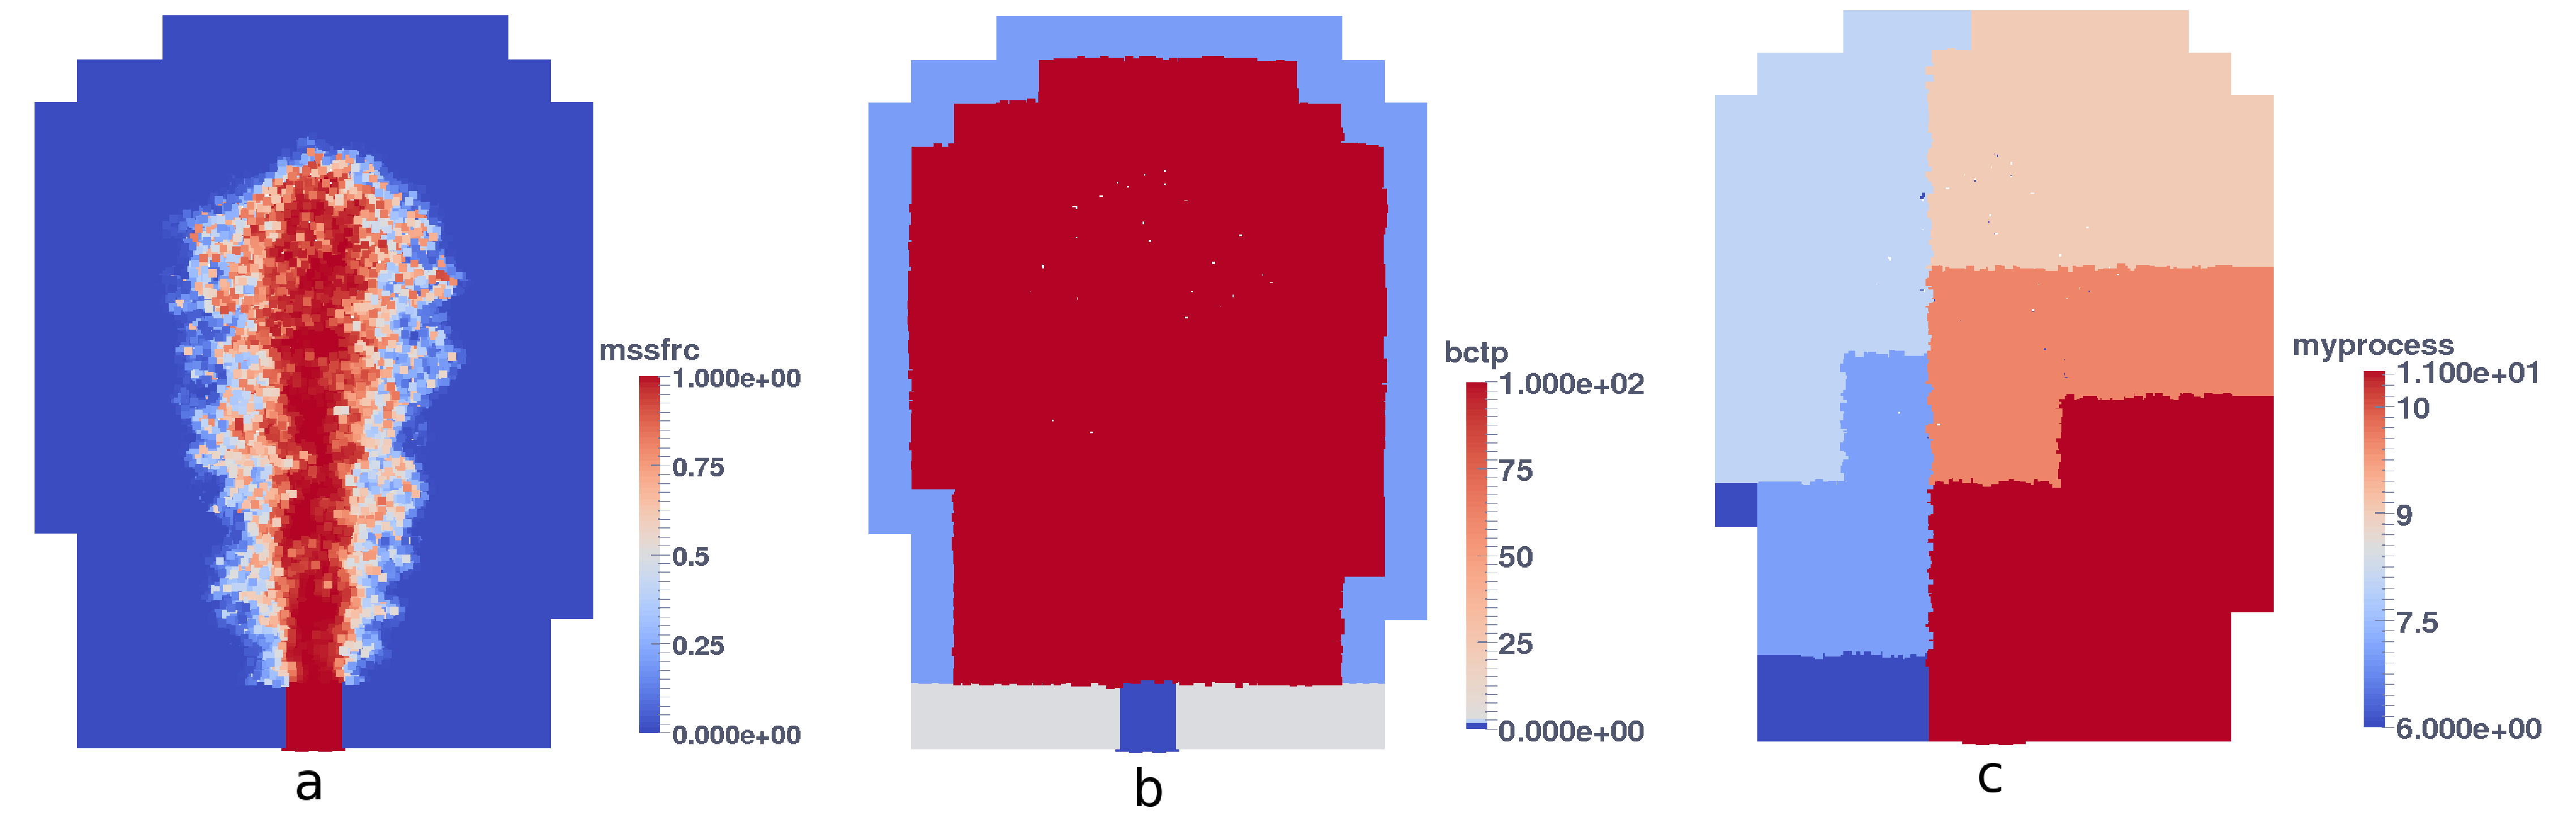
\includegraphics[width=18cm]{Chapter-3/Figures/t120_bc_proc}
\caption{A cross section view of the simulation domain in $y-z$ plane at 66 seconds. Subfigure $a$ shows the mass fraction. Subfigure $b$ shows all boundary conditions: the dark blue region are occupied by eruption ghost particles with "Ghost particle ID" of 0, the light blue area are occupied by pressure ghost particles with "Ghost particle ID" of 1, the gray area is filled with wall ghost particles with "Ghost particle ID" of 2, "Ghost particle ID" of all real particles are set to 100, they occupy the major portion of the domain in subfigure $b$. Subfigure $c$ shows the cross section view of domain decomposition based on SFC. The simulation is conducted on 12 processors, so there are 12 subdomains in total. The crosss section view shows a portion of them.}
\label{fig:bc_and_domain_decomp}
\end{figure}
%%%%%%%%%%%%%%%%%%%%%%%%%%%%%%%%%%%%%%%%%%%%%%%%%%%%%%%%%%%%%%%
% Appendices
%
% Because of a quirk in LaTeX (see p. 48 of The LaTeX
% Companion, 2e), you cannot use \include along with
% \addtocontents if you want things to appear the proper
% sequence. Since the PSU Grad School requires
%%%%%%%%%%%%%%%%%%%%%%%%%%%%%%%%%%%%%%%%%%%%%%%%%%%%%%%%%%%%%%%
\appendix
\Appendix{Post processing of particle data}

\label{app:project-SPH-grid}    %% Appendix A
%\appendixfigures
\begin{figure}[!htb]
    \centering
	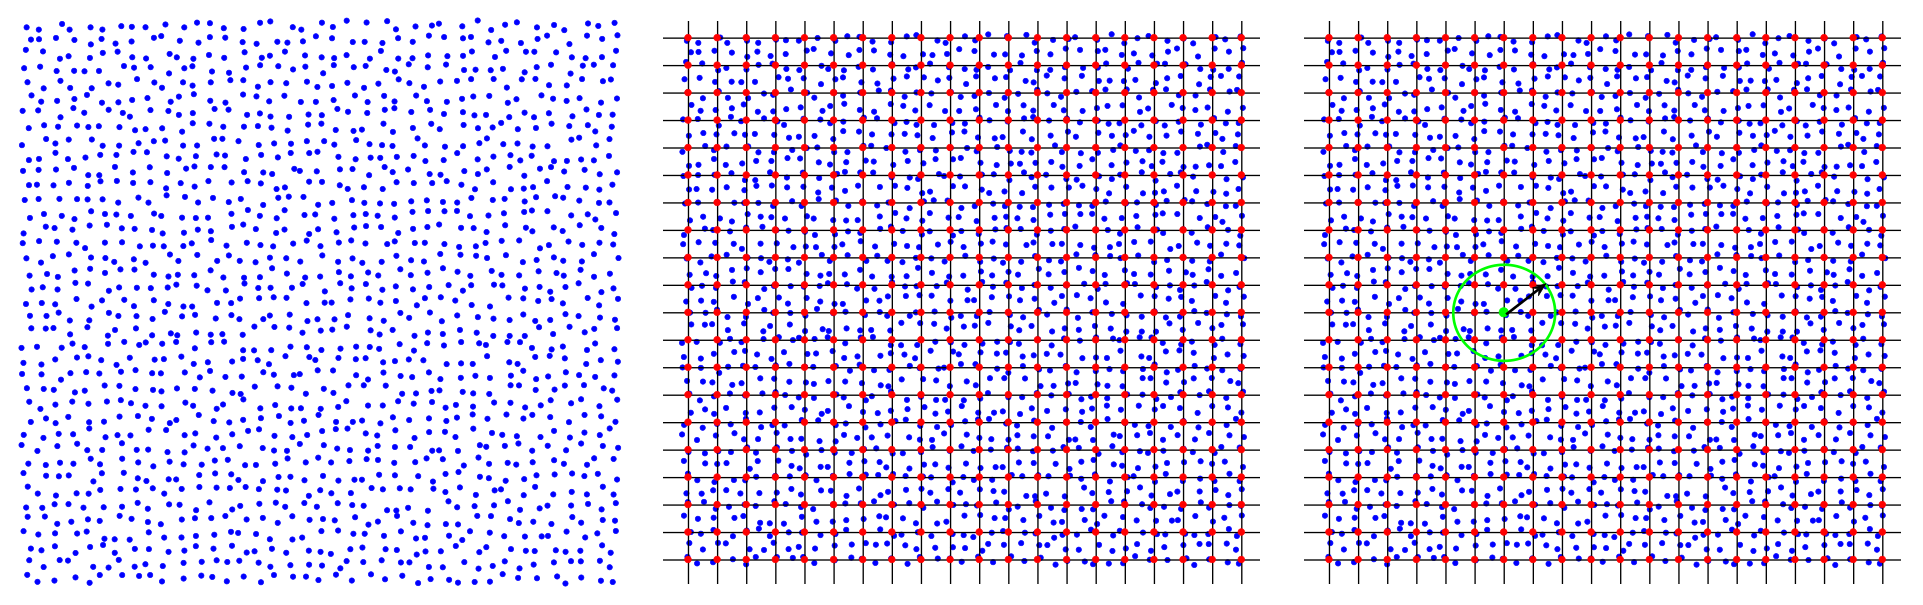
\includegraphics[width=14cm]{Appendix-A/Figures/FigA1.png} 
    \caption{Procedure of projection of simulation results carried by particles onto regular grids. as shown in these figures from left to right: 1) raw data of SPH simulation results (irregularly distributed in space), 2) Add regular mesh, 3) searching for neighbours of each node (the blue SPH particles within the green circle around the red dot). The last step is not shown in these pictures, which is treating each node on the regular mesh as a SPH particle and projecting data on particles onto nodes utilizing "SPH interpolation" ( see Eq. (\ref{eq:SPH-fundamental-principle})).}
    \label{appfig:1D-shock-tests-verification}
\end{figure}

Particles distribute irregularly in SPH simulation results. To adapt post processing originally proposed for mesh-based method, we need to project simulation results onto a pre-defined regular mesh. As shown in Fig. \ref{appfig:1D-shock-tests-verification}, the basic steps for such projection are:
\begin{itemize}
\item obtain raw simulation results carried by particles that irregularly distribute in the space
\item create regular grids
\item search for neighbour paricles for each node of the regular grids.
\item interpolate physical quanties from neighbour particle onto corresponding node of regular grids according to Eq. (\ref{eq:SPH-fundamental-principle})
\end{itemize}
\Appendix{DOI Afterthoughts}

\section{Introduction}
When in the Course of human events, it becomes necessary for one people  to dissolve the political bands which have connected them with another,  and to assume among the powers of the earth, the separate and equal station  to which the Laws of Nature and of Nature's God entitle them, a decent respect to the opinions of mankind requires that they should declare  the causes which impel them to the separation.

\section{More Declaration}

We hold these truths to be self-evident, that all men are created equal,  that they are endowed by their Creator with certain unalienable Rights,  that among these are Life, Liberty and the pursuit of Happiness. --That to secure these  rights, Governments are instituted among Men, deriving their just powers  from the consent of the governed, --That whenever any Form of Government  becomes destructive of these ends, it is the Right of the People to alter  or to abolish it, and to institute new Government, laying its foundation on  such principles and organizing its powers in such form, as to them shall  seem most likely to effect their Safety and Happiness. Prudence, indeed, will dictate that Governments long established should not  be changed for light and transient causes; and accordingly all experience  hath shewn, that mankind are more disposed to suffer, while evils are  sufferable, than to right themselves by abolishing the forms to which they  are accustomed. But when a long train of abuses and usurpations, pursuing invariably the same  Object evinces a design to reduce them under absolute Despotism, it is their  right, it is their duty, to throw off such Government, and to provide new Guards for their future security. --Such has been the patient sufferance of these Colonies; and such is now the  necessity which constrains them to alter their former Systems of Government.  The history of the present King of Great Britain [George III] is a history  of repeated injuries and usurpations, all having in direct object the  establishment of an absolute Tyranny over these States. To prove this, let Facts be submitted to a candid world.
%%%%%%%%%%%%%%%%%%%%%%%%%%%%%%%%%%%%%%%%%%%%%%%%%%%%%%%%%%%%%%%
% ESM students need to include a Nontechnical Abstract as the %
% last appendix.                                              %
%%%%%%%%%%%%%%%%%%%%%%%%%%%%%%%%%%%%%%%%%%%%%%%%%%%%%%%%%%%%%%%
% This \include command should point to the file containing
% that abstract.
%\include{nontechnical-abstract}
%%%%%%%%%%%%%%%%%%%%%%%%%%%%%%%%%%%%%%%%%%%
} % End of the \allowdisplaybreak command %
%%%%%%%%%%%%%%%%%%%%%%%%%%%%%%%%%%%%%%%%%%%

%%%%%%%%%%%%%%%%
% BIBLIOGRAPHY %
%%%%%%%%%%%%%%%%
% You can use BibTeX or other bibliography facility for your
% bibliography. LaTeX's standard stuff is shown below. If you
% bibtex, then this section should look something like:
   \begin{singlespace}
   \bibliographystyle{apsr}
   \addcontentsline{toc}{chapter}{Bibliography}
   \bibliography{dissertation}
   \end{singlespace}

%\begin{singlespace}
%\begin{thebibliography}{99}
%\addcontentsline{toc}{chapter}{Bibliography}
%\frenchspacing

%\bibitem{Wisdom87} J. Wisdom, ``Rotational Dynamics of Irregularly Shaped Natural Satellites,'' \emph{The Astronomical Journal}, Vol.~94, No.~5, 1987  pp. 1350--1360.

%\bibitem{G&H83} J. Guckenheimer and P. Holmes, \emph{Nonlinear Oscillations, Dynamical Systems, and Bifurcations of Vector Fields}, Springer-Verlag, New York, 1983.

%\end{thebibliography}
%\end{singlespace}

\backmatter

% Vita
\vita{SupplementaryMaterial/Vita}

\end{document}

